%%%%%%%%%%%%%%%%%%%%%%%%%%%%%%%%%%%%%%%%%%%%%%%%%%%%%%%%%%%%%%%%%%%%%%%%%%%%%%%%
%
% Purpose: abstract for orientation model
%
% 
%
%%%%%%%%%%%%%%%%%%%%%%%%%%%%%%%%%%%%%%%%%%%%%%%%%%%%%%%%%%%%%%%%%%%%%%%%%%%%%%%%

\chapter*{Executive Summary}
The \ModelDesc forms a component of the utilities suite of models
within \JEODid. It is located at models/utils/orientation.

This document describes the implementation of the \ModelDesc including
the model requirements, specifications, mathematical theory,
and architecture.  A user guide is also provided to assist
with implementing the model in Trick simulations.

\section*{Rotations in JEOD}
There are many ways to represent the orientation of one three dimensional
object with respect to another. The representation schemes supported in JEOD are
\begin{itemize}
\item Special orthogonal matrices, or proper rotation matrices.
A proper rotation matrix is an orthogonal matrix whose determinant is one.
The Matrix3x3 class in the \hypermodelref{MATH} provides methods for
manipulating 3x3 matrices and for using them to transform 3-vectors.
Note that JEOD uses transformation matrices rather than rotation matrices.
\item Unit quaternions.
The unit quaternions are the subject of the \hypermodelref{QUATERNION}.
The Quaternion class defined in that model provides methods that relate to
using unit quaternions to represent rotations and transformations.
Note that JEOD uses left transformations unit quaternions exclusively.
\item Eigen axis, or single axis, rotations.
Any sequence of rotations in three dimensional space is equivalent to
a pure rotation about a single axis.
JEOD represents eigen rotations in terms of a rotation angle (a scalar) and a
unit vector that defines the direction of the rotation via the right-hand rule.
\item Euler rotations. An Euler rotation sequence is a sequence of three
rotations about a set of principal axes. There are twelve possible conventions
for these rotations. JEOD implements all twelve conventions.
\end{itemize}

\begin{figure}[hbtp]
\centering
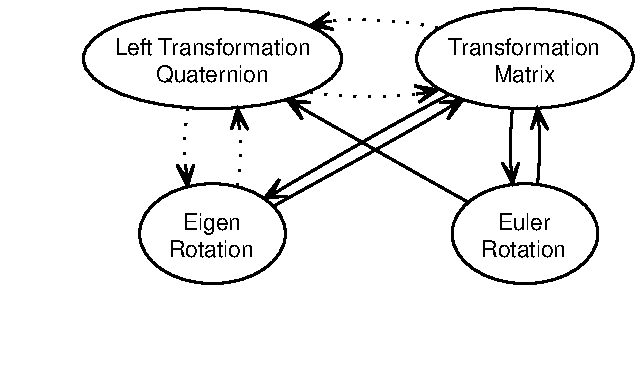
\includegraphics{representations}
\caption{Orientations in JEOD}
\label{fig:summary_representations}
\end{figure}

Figure \ref{fig:summary_representations} portrays these four representation
schemes and the direct conversions between them provided by \JEODid.
The dotted lines represent conversions implemented by the \QUATERNION~while
the solid lines represent conversions implemented in this model.

\section*{Model Architecture}
This model exists for two reasons. One reason is to provide those conversions
represented as solid lines in figure~\ref{fig:summary_representations}.
The other reason is to provide an input mechanism by which a user can specify
a rotation or transformation using any of the representation schemes described
above. The Orientation class provides both of these capabilities.

The class provides a static method for each of the conversions represented
as a solid line in figure~\ref{fig:summary_representations}.
Note that the graph in figure~\ref{fig:summary_representations} is not
fully connected.  While it is possible to convert between any two representation
schemes, some conversions require the use of an intermediate representation
scheme. For example, converting a left transformation quaternion to an Euler
rotation sequence requires going through a transformation matrix as an
intermediate step.

The Orientation class is also instantiable. An Orientation object contains data
members that correspond to each of the four representation schemes supported by
JEOD and contains auxiliary data members that indicate which representation
scheme was input by the user. Other JEOD models can query the Orientation object
to express the user-input data in any of the four supported representations.

\section*{Interactions With Other Models}
Four of the conversions in figure~\ref{fig:summary_representations},
the conversions between quaternions and matrices
and the conversions between quaternions and eigen rotations,
are represented as dotted lines.
The Quaternion class in the \QUATERNION~provides the methods that implement
these conversions.
